\documentclass[11pt]{article}
\usepackage[top=1.00in, bottom=1.0in, left=1in, right=1in]{geometry}
\renewcommand{\baselinestretch}{1.1}
\usepackage{graphicx}
\usepackage{natbib}
\usepackage{amsmath}
\usepackage{multicol}
\usepackage{tcolorbox}
\usepackage{caption}
\usepackage{todonotes}

\bibliographystyle{besjournals}

\begin{document}

\title{Closing the gap between statistical and scientific workflows for improved forecasts in ecology } 
\date{\today}
\author{Victor Van der Meersch, J. Regetz, T. J. Davies \& EM Wolkovich}
\maketitle

{\bf Deadline:} 1-ish May 2025 (was 1 April 2025, getting in by May 8th would be good!)

\emph{For:} Scientific and Statistical Workflow theme issue for \emph{Phil Trans A} as an \emph{Opinion}
% They mention a tex template here: https://royalsocietypublishing.org/rsta/for-authors#question4
% Word length: I should check what they emailed but they say no more than 13 printed pages with 650 per page (whoa, we should be well below that! I am thinking 3-5K would be good)
% Already 5K! 

% Jim, if you want to add any of this into the abstract, please do!
%There's a fundamental problem in how a lot of empirically but observationally driven (i.e., non-experimental) research is done in ecology and related fields. The crux of the issue comes down to a couple of things. First, the research community has two very distinct paradigms for modeling the system or phenomenon or interest: either fitting simple trend-like models with only one or a few parameters, or developing forecast models that often include potentially complex, mechanistic, and/or black box submodels largely unconstrained by data. Second, regardless of the approach, these models tend to be developed not only in isolation of one another, but also without a coherent strategy for linking modeling/statistical decisions, data, and scientific understanding (both as input and output) throughout the entire modeling process. We propose a unified, principled workflow for end-to-end empirical model development, incorporating sound statistical and scientific practices, and especially relying on data simulation to inform decisions at multiple steps in the process.

\begin{abstract}
Increasing biodiversity loss and climate change have led to greater demands for useful ecological models and forecasts. Relevant datasets to meet these demands have also increased in size and complexity, including in their geographical, temporal and phylogenetic scales. While new research often suggests that accounting for these complexities has a major impact on projected trends and forecasts, we argue that the typical approach to model fitting in ecology makes it impossible to evaluate and compare the models used to generate these insights and predictions. % jdavies15april: I feel this could be a critical step somehow - sharing simulations could allow cross-validation between models or perhaps cross-calibration ...
These problems stem in part from continuing gaps between statistical workflows---where the data processing and model development are often addressed separately from the ecological question and aim---and scientific workflows, where all steps are integrated. Yet, as ecologists become increasingly computational the opportunity to close this gap has never been greater. We outline how increased data simulation at multiple steps in the scientific workflow could revolutionize our understanding of ecological systems, yielding new insights for both trend estimation and forecasting.
%Combining these changes with more open model and data sharing---and developing new efforts to race the same data---could be transformative for ecological forecasting. 
A shift toward universal training in a more robust model building could bridge the gap between process-based and statistical approaches and be transformative for ecological modeling.
\end{abstract}

{\noindent \bf Goal:} Increase awareness of how we can merge statistical and scientific workflows in ecology (especially forecasting) and what we would get out of it.
\vspace*{0.5cm}

\section{Introduction}

Anthropogenic drivers are reshaping natural systems \citep{Diaz2019}. Impacts are projected to increase in coming decades, as climate change accelerates biodiversity loss, altering ecosystem services and human well-being \citep{IPBES2019}. % jdavies15april: not sure what models you are referring to here, but perhaps look up models of 'mean species abundance'.
Implementing sustainable policies to mitigate these impacts is thus a global priority, but designing the best policies requires estimating and understanding biodiversity and ecosystem trends to date alongside the skill to forecast future dynamics. % These requirements in turn have created a growing need for more global ecological data, and the types of models that can robustly handle such data. 

Meeting these policy needs has led often to two separate paths: one focused on estimating trends from new global datasets and another focused on forecasting from generally distinct datasets or mechanistic models based on less data. Newly available large-scale, long-term datasets have provided our first `global' estimates of biodiversity trends \citep[e.g.][]{loh2005living,Dornelas2018}, but these data---gathered opportunistically from multiple sources---are unbalanced with massive geographic, temporal and taxonomic biases. Models to date have failed to fully address these challenges and, perhaps because of these limitations, are rarely if ever used for forecasting. 
Instead forecasting---under different plausible scenarios---has generally relied on entirely different datasets combined with either correlative or process-based models \citep{IPBES2019}, with process-based models often promoted as the most realistic approach \citep{Urban2016, Pilowsky2022} because they focus on mechanistic representations of ecosystem functioning. The current outcome from these approaches is no clear agreement on current species trends, with ongoing debates on the magnitude and even direction \citep{Dornelas2014, Leung2020, Buschke2021, Johnson2024}, and forecasts that diverge due to high model uncertainty at the ecological level \citep{Cheaib2012}. 

We argue that current debates and diverging forecasts are driven in large part by the incoherent and disconnected workflows used today in ecology \citep{Loreau2022, Talis2023, Johnson2024}. Research estimating biodiversity trends has become focused on methodological aspects because the current workflow fails to examine the gap between ideal and available data, and rarely tests for predictive accuracy that could scale up to allow forecasting. At the same time, forecasting-focused process-based models often develop by adding new separate layers or components. These new parts are often disconnected from the original research aim, its data stream and the previous scientific insights, because current approaches rarely examine the model as a functioning whole and thus ignore major problems (e.g., non-identifiability, discussed below). 

Workflows that fully integrate all the steps required to build a model from an ecological question, evaluate its limitations and potential problems, before estimating its parameters and making projections, could reduce many of these problems. In particular, we argue that workflows that incorporate data simulation at multiple steps can quickly identify flaws in model structure and constraints in data, and allow us to understand when, where and why different models diverge. Towards this aim,  we outline the steps of a universal workflow that could harmonize both trend estimation and forecasting.

\section{Scientific method and workflows}

Quantitative science relies on a model-based framework, to confront hypothesis with data \citep{Chamberlin:1965cd}. In an idealized scientific method, we would formulate a research question and hypotheses, design an experiment accordingly, build a model, collect data, and using this data to inform our model and differentiate between hypotheses. This method underlies much of the recent pre-registration movement, where hypotheses and methodology are defined prior to data collection. %add cites for prereg?
But this idealized method often does not apply to the reality of ecological research. Many important questions cannot be addressed through controlled experiments and replications. Instead, we must often rely on existing, heterogeneous datasets alongside uncertain and incomplete theory to provide a large-scale and long-term perspective \citep{Hilborn1997}, and most of macroecological insights emerge from exploring patterns in these datasets (exploratory data analysis).

This reality should drive researchers to use more robust and coherent methods. But the current workflows combined with the challenges ecologists are facing---both in term of data complexity and societal needs---instead may lead to persistent problems. % jdavies15april: what challenges? forecasting from imperfect data or the urgent need to generate forecasts?
Trend estimation has focused mostly on fitting a model to empirical data in a uni-directional way---without the checks and likely feedbacks that often highlight uncertainty and related limitations in the model and/or data (Fig. \ref{fig:modeldata}). For forecasting, researchers have focused on making predictions with increasingly complex mechanistic models, frequently obscuring the steps underlying model building and parameterization (Fig. \ref{fig:modeldata}). Researchers often calibrate the different parts of these models separately, and fix some parameter values based on experiments and expert knowledge, to avoid problems when trying to fit the model as a whole. % jdavies15april: is this particularly specific to process based models? 
Addressing these problems while accounting for the realities of working with ecological data requires a more comprehensive workflow. 
% mention the disconnection between trends and forecasts?

\begin{figure}[h]
	\centering
	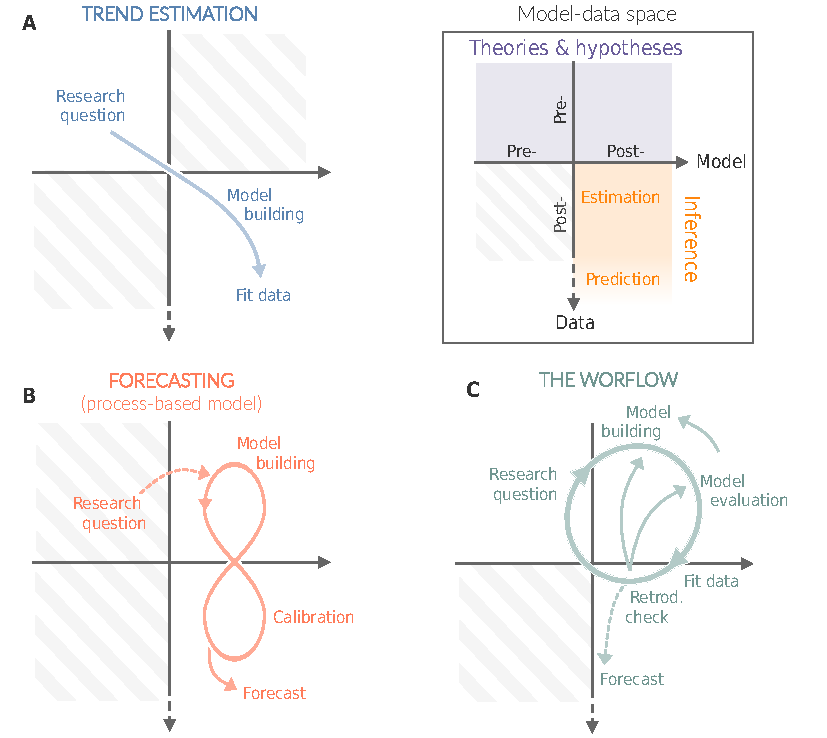
\includegraphics{figures/modeldataspaces_rotation}
	\caption{Here the caption could explain a bit more the pre-model pre-data to the post-model post-data...} 
	\label{fig:modeldata}
\end{figure}
% jdavies15april: Could the bottom right be where exploratory data analysis fits in, generating hypotheses that inform the research question?

We argue a workflow that moves along the data-model space in a coherent sequence of steps with repeated data simulation % jregetz16april: Maybe “data simulation” needs to appear in the figure? Or wait to mention simulation until referencing Fig 2? [FLAG: what do you think? I agree you should choose on of the two options]
(Fig. \ref{fig:modeldata}c) could reduce many of these problems and thus improve ecological science.
The first step of this workflow is to define an explicit research question and formulate hypotheses (step 1, fig. \ref{fig:workflow}). This involves making clear assumptions about the most influential drivers, within the specific context of our study. This step should guide the construction of a narrative model of how we believe the system works, focusing on the mechanisms that could generate the data we observe, including the observational error. % vvdm16april: to answer Jonathan comment about verbal model
From this narrative, we can then develop a mathematical model---an ensemble of equations that encapsulates our knowledge and is designed to answer our research question (step 2, fig. \ref{fig:workflow}). The general idea is to start with a relatively simple model that we could refine later. At this stage, prioritizing biologically meaningful parameters is crucial, as it allows us to have a sense of plausible parameter values. This means choosing a model formulation where each parameter corresponds to an interpretable behavior (which sometimes requires considering alternative parameterizations).

With a model in place the next step focuses on testing and understanding it via data simulation (step 3, fig. \ref{fig:workflow}). `Fake' or `test' data are generated directly from the model by fixing parameters to some reasonable range of values (which is straightforward if the parameters are interpretable) and from fake predictor data. % This simulated data should reflect the full model assumptions, and could begin to include complexities in our data structure and biases, which may in turn lead to adjusting the model. % jdavies15april: I think you could introduce this as a separate step as it seems there is a tendency for people to want to do this immediately (i.e. simulate fake data that looks like their data - I am looking at Max and Isidora ...), but I don't think this is helpful when first structuring a model. [FLAG: yes I can understand this point...]
% For example, if a researcher realizes their empirical data is geographically biased, then this bias should be built into the model and thus then into this data simulation step. [FLAG: so I moved this sentence below, when we say "Insights from the retrodictive check can also lead us to introduce additional complexity when simulating fake data"
We then fit our model to this simulated dataset and evaluate its ability to recover the prescribed values. At this stage the focus is understanding the model, so researchers may have to spend a while to think through what parameters are reasonable or not. This is also a step for making sure the model is working as we expect, so simulated data often would have low error and high sample sizes (to make sure the model returns the parameter values used to generate the simulated data), 

Once we are confident about our model structure, we can introduce real data as part of an initial model fitting step (step 4, fig. \ref{fig:workflow}). This way, we obtain parameter estimates constrained by observations. 
%emwApr19: I commented out the below as I think linking difficulty in fitting the model to problems with the data is pretty tricky (difficulty in fitting the model can point to many things!) and thus too confusing to include here. 
% Here, difficulty in fitting the model might indicate an inherent need for more data to address our initial question, or re-evaluate the model of how we think the system works. This could lead us to either simplify our research question or---ideally---launch new data collection efforts. 
These parameter estimates lead to the second data simulation step, this time using our fitted model parameters to generate predictions (step 5, fig. \ref{fig:workflow}). This retrodictive check allows model output to be compared to observations. % jregetz16april: do we need to define “retrodictive”?
% The workflow encourages a focus on the full model, and replaces parameters at the core of the modeling process, as fundamental components that shape both inference and forecasting. % jregetz16april: Not sure what this means? jdavies did not like it either! (he thought it was a typo), vvdm16april: reformulate:
The workflow encourages a focus on the full model, where any parameter (such as a trend estimate) must be carefully interpreted alongside others, as all are fundamental components that shape both inference and forecasting. 
Within such a workflow, forecasting emerges as a natural outcome: rather than being a final goal, it only involves jointly modeling new circumstances along with the original data. The adoption of the workflow in macroecological studies---where model building is often informed by patterns in the data---would also make the exploratory analysis more transparent (as an explicit preliminary step for entering the workflow) and would compel researchers to more clearly develop a research question before extensive model fitting. 

\begin{figure}[h]
	\centering
    \hspace*{-1.5cm}
	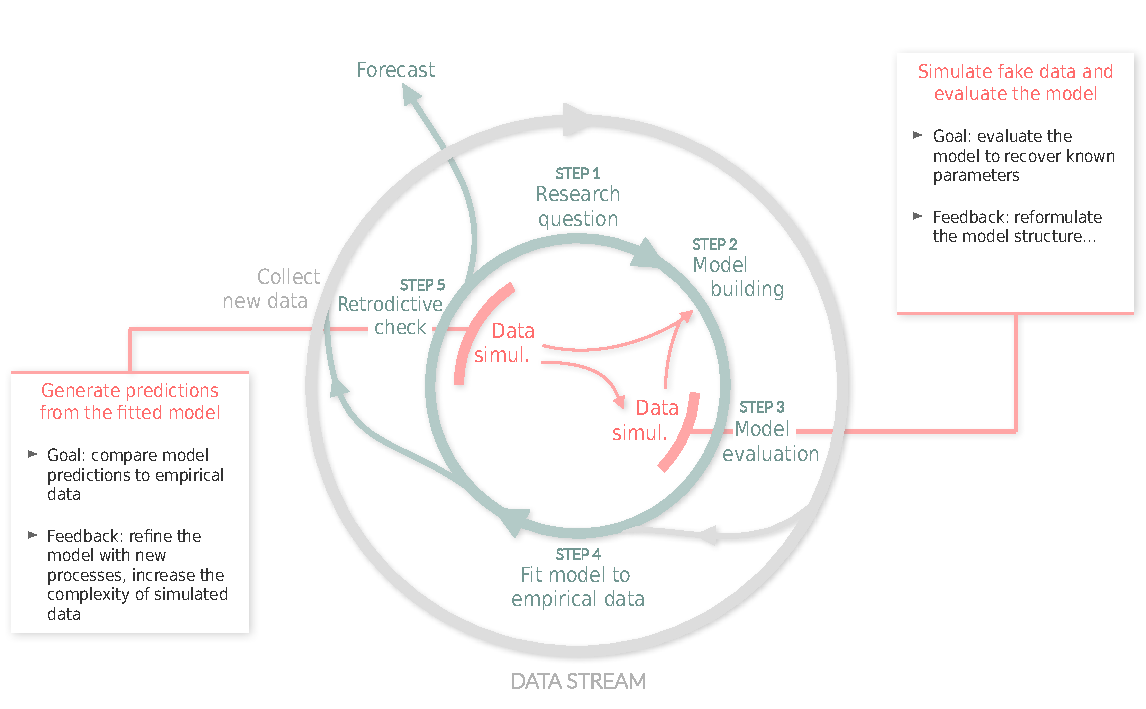
\includegraphics{figures/figure_worflow_wsteps}
	\caption{Here we could have a caption like ... Our workflow builds on others (with citations) to highlight the integrated nature of stuff in ecology. We can work on this once we get feedback from mighty co-authors. Also, should we list the steps on the figure? What do people think?} 
	\label{fig:workflow}
\end{figure}

% More details, what's special! Feedbacks!
A key feature of this workflow is the central role of data simulation, which introduces two feedback loops. The first feedback arises when we evaluate the model on simulated data.
The failure of the model to recover known parameter values and handle the complexity of the simulated data should prompt a reconsideration of the model, or even a reformulation of the research question.
Further, this step might reveal that some parameters are highly non-identifiable (meaning the parameter(s) cannot be uniquely estimated),
flagging the need to change the model structure---before incorporating real observations. 
The second feedback loop comes from the retrodictive check. 
Discrepancies here may indicate a missing key driver, and suggest the current model is too simplistic. We can refine the model to integrate the missing process(es) (if we can identify them) and restart the workflow. Insights from the retrodictive check can also lead us to introduce additional complexity when simulating fake data, such as phylogenetic structure or observational biases (e.g. unbalanced data). For example, if a researcher realizes their empirical data is geographically biased, then this bias should be built into the model and thus then into this data simulation step. This iterative evaluation of the model moves beyond a simple reliance on goodness-of-fit metrics. At each iteration, we are able to evaluate the model behavior, both with simulated and real data, taking into account our expert knowledge of the ecological processes. 

\section{The workflow in practice}

%emw6Apr: I like the shift to 'parameter estimation' instead of trend estimation, but I wonder if we could make that shift clearer above. Maybe somewhere we say that the workflow would  encourage a focus on the full model and its parameters: For trend estimates, the trend becomes just one parameter that must be carefully interpreted alongside others . 
Across the different fields of ecology---for both parameter estimation and forecasting---a systematic application of a coherent workflow could highlight the best opportunities to reduce uncertainties through new scientific insights, toward the most critical steps. This will help refocus the debate on designing new hypothesis, formulating new questions---and guiding efforts to collect new data. Here, we illustrate how such a workflow could lead to significant improvements in two case studies: (i) estimating global biodiversity trends and (ii) forecasting future species and ecosystem dynamics using process-based models.

\subsection{Trends}

%jregetz16april: One thing I’m stuck on (and could’ve written this note earlier too). Is “trends” really essential? Or is this just shorthand for “simple, one/few parameter, non-mechanistic forecasting models”? If yes, can we generalize that in the MS overall, or at least say so up front and then say e.g. “we’ll refer to these as trend models for brevity”? If no, and something about trend estimates is specifically key to the paper, can we say more about *that*? [FLAG]
%emwApr19: I think the only key part is that biodiversity trends and trends over time are big in forecasting ... as long as we don't lose that I think it would be great to make the suggested change -- Jim, can you see if you can edit it on the next round? 

Ecologists today have amassed data on populations and species across the globe; they have also engaged in an increasing number of debates on regional and global trends over time, with arguments over the magnitude and even direction of population and biodiversity metrics \citep{Dornelas2014,Leung2020,terry2022no,muller2024weather}. While shifting estimates are part of the process of science---refining our approaches and thus estimates over time---we believe these debates would be much reduced and more rapidly resolved through use of an improved workflow. % Further, an improved workflow could give more rapid and coherent estimates, which could make it easier for  policy-makers to develop and advance initiatives aimed at slowing declines.

An improved workflow that required data simulation and retrodictive checks would lead to larger model advances and a greater recognition of uncertainty---thus highlighting likely consistency in estimates across models---that could better aid policy.  Using the workflow would make what now appear as major discrepancies more obviously shifts in point estimates that are generally all in the same uncertainty space \citep{Johnson2024}---and it would challenge modelers to show major predictive advances, which is not currently part of the process. Explanatory power in most models of observational data is usually very low \citep{low2014rising,moller2002much} and thus tests of models' predictions rarely expected. But the workflow highlights that predictions from the model---what we call retrodictive checks---are part of the process of science, and critical to testing for what may be missing in a model. We expect retrodictive checks on most published trend analyses would highlight major missing components in these models, and drive changes both in the models themselves and in the simulated data to check the models. This step builds somewhat on the skills needed for null models \citep{Gotelli:2012oz}, but with a shift in focus towards the specific bespoke model at hand. Ecologists have started to use simulated data more to understand potential limitations of their models and data combined, but this is still extremely rare, and efforts to date often treat simulations as separate from the statistical model \citep{Buschke2021,dove2023quantifying}, short-circuiting their full utility if used in an iterative workflow. 

% expand on 'highlight major missing components in these models'? ADD example?
% Simulating data to verify and test models in trend analyses is currently rarely reported, which we believe makes it easier for ecologists to fit poor models and in turn debate them.. 
% Mention elephants rebounding...

% Trends - improvements!
Applying the workflow to current trend estimates could importantly highlight the best way to improve data collection for more reliable estimates. Returning to the example of a global estimate of trends in vertebrate populations of species over time and applying our proposed workflow would mean more efforts to define the goal and question---is it a simple global estimate? % jdavies15april: This is what the LPI wants to be (like a index fund in the stock market tracking trends over time) , but this is often overlooked.
Or a need to also find which species are declining most, including those that may have poor or no data? From there a generative model using simulated data for testing could incorporate many aspects of the populations, and data, that are often only included in `null' or 'synthetic data generation' currently \citep{Buschke2021,mcrae2025utility} but could be built into the models fit to the empirical data. Eventually fitting the empirical data and performing retrodictive checks would likely highlight major missing components of the generative model and, ultimately, this would help inform our global estimates of mean trends. For example, certain populations are recovering for very specific reasons (e.g., elephants in regions where the ivory trade drove declines in the past) that perhaps should be modeled. From this model, what data are most critically needed to address the updated aims would become clearer and could drive new data collection \citep{toszogyova2024mathematical}. 

\subsection{Forecasting from process-based models}

Ecological forecasting is a broad field with a diverse range of methods. Our second case-study focuses on process-based modeling, which is often considered the gold standard for forecasting in ecology \citep{Urban2016, Pilowsky2022} and beyond. Newer models generally incorporate greater complexity and an ever-growing number of parameters, making it more difficult to increase scientific understanding \citep{Franklin2020}, and suggest or model potential policies. 

Increasing model complexity can be beneficial, especially when it reduces uncertainty; however, this is not always the outcome. In process-based modeling for climate forecasts, the uncertainty range on the effect of increasing CO$_{2}$ concentration on temperature have remained largely unchanged \citep{Zelinka2020}. This has driven calls for more rigorous and transparent calibration processes \citep{balaji2022general}. Similar concerns arise in ecology, where strong disagreements exist about the effect of climate change on future species distributions \citep{Cheaib2012} and ecosystem dynamics \citep{Lovenduski2017}.
These uncertainties have large implications beyond ecology, as they influence simulations of biosphere-atmosphere interactions and, ultimately, future climate projections \citep{Bonan2018, simpson2025confronting}.
Some researchers now advocate for the simplification of models, to avoid over-parametrization when the data provide little information to constrain some parameters \citep{Wang2017, Harrison2021}. \todo[size=\tiny]{jdavies15april: need to distinguish this from multiple model comparisons that attempt to identify the 'minimum adequate model' - which lead to overfitting. Reply: we agree but not really relevant to PBM? Maybe it's not clear enough we are focusing on PBM in this section, which we tried to change above, see if it works}
If a model becomes too complex, it may become a black box, % mention black box here to line up with the beginning of next paragraph
and understanding the sources of uncertainty and how they propagate through the model may become nearly impossible.
Each additional process and parameter can increase overall uncertainty to the point where model projections lose their usefulness for decision makers \citep{Saltelli2020}. \todo[size=\tiny]{jdavies15april: complexity, such as interaction terms also requires more data to fit, and thus adding parameters can increase parameter uncertainty .... Reply: Same as just above.}

Process-based models used to project species or ecosystem distributions highlight some of these problems. Most of the focus is on the model projections---often represented as maps without uncertainties. Model evaluation generally focuses on how well these projections match observed distributions, sometimes under different climatic conditions to challenge the models \citep{VanderMeersch2025a}---most of the time evaluating only one of the many different output variables of the model. %The model building and calibration steps are usually limited to the Methods section, and estimated parameter values are rarely discussed \citep[e.g.][]{Conradi2024, VanderMeersch2025a}. 
The complexity of these models often makes it difficult to assess how well the potential parameter space was searched, and whether there was any potential non-identifiability---such work is generally done as a separate effort, exposing potential model problems later on \citep{VanderMeersch2025b}, and not required as a preliminary step. \todo[inline, size=\tiny]{For above, addressing: jdavies15april: it would be nice to also have a clear empirical example (like the LPI above) in this section - are we projecting species distributions, ecosystem properties? This could help illustrate potential degeneracies etc. Reply: Tried something, but not sure it works so feedback much appreciated!} 

%emw19Apr -- Can we just get away with using non-identifiable and save the reader also needing to digest degenerate? (https://betanalpha.github.io/assets/case_studies/identifiability.html)? I tried that on this draft, see how it works!
Applying the workflow to process-based models would help open the black box.
Each successive step of model development in the workflow may highlight current problems and a path to solutions. Incorporating data simulation would introduce a crucial step between model building and data fitting (also called calibration), ensuring a clear delineation between the two and help expose potential parameter identifiability issues in the model design. %jregetz16april: Maybe good to define the term degeneracy here (like we do for non- identifiability below) 
Uncovering identifiability issues would likely force researchers to begin with a simpler version of the model, which they could build on iteratively, testing for support---or lack thereof---when adding model complexity. The workflow may also highlight model problems by requiring more explicit model calibration (i.e. data fitting), % jdavies15april: still not really sure what is 'model calibration' and how it differs from model fitting and parameter estimation
which is currently hidden within opaque `model building', making it easy to hide non-identifiability in the model. Through the workflow non-identifiable parts of models could be addressed by reformulating the mathematical structure of certain processes, or finding ways to apply additional constraints (e.g., narrower ranges for certain parameters or developing new hypotheses that target the appropriate level of complexity). The resulting process-based models would likely be simpler and thus more tractable for quantifying parameter uncertainty and propagating it through projections. 

\todo[inline, size=\tiny]{For below: jdavies15april: might be better grouped together in concluding section. Reply: if we want to put this in the concluding section, we would need to talk also about the "opportunities to bridge statistical and process-based", rather than keeping it in the box? So, what should we put in the box?}
Beyond improving the model building, the workflow also has the potential to shift how process-based models are perceived, particularly by those unfamiliar with them. The workflow could refocus attention on the research question, highlighting the ecological hypotheses that justify the use and design of the model. It would thus define a clear and limited context in which the model should apply, without always arguing about the necessity of adding more and more complexity.  % or something like : "rather than driving a constant push for increasing complexity" --- my idea is that people are always like : "oww, your model is nice, but you should add [whatever they are working on]" (classical example I heard few times: mycorrhiza! disease! pathogens!)... or "rather than constantly expanding models by adding ever more processes"? 
Process-based model would once again be a way to answer a research question---whereas today, model simulations have increasingly become a subject of study on their own.
Ideally, applying the workflow would help to move away from the traditional process-based model paradigm, where parameters are typically assigned fixed values without properly accounting for their uncertainty. Instead, it would guide a step-by-step model fitting, parameter estimation, and uncertainty quantification. 

This shift would present a significant challenge---as it would likely reveal many issues related to non-identifiability in models and data limitations before achieving robust inference. But ultimately, it would prevent modelers from making biased inferences and unfounded assumptions beyond what the data can support. 


% Box
% \setlength{\columnseprule}{0.1pt}
\begin{tcolorbox}[
sharp corners=all,
colback=white,
colframe=black,
size=tight,
boxrule=0.1mm,
grow to left by=+1cm, grow to right by=+1cm,
enlarge top by=-1.2cm,
left=3mm,right=3mm, top = 2mm, bottom = 2mm,
fontupper=\footnotesize
]
{\begin{multicols}{2}

\centerline{\bf Trend estimation}
\vspace*{2mm}
\begin{minipage}[t]{\linewidth}
    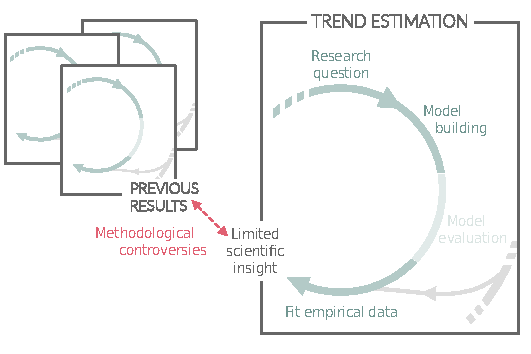
\includegraphics[width=\linewidth]{figures/trendestimation_details}

    % \vspace{-0.5cm}\captionsetup{font=footnotesize}\captionof{figure}{Caption}\label{fig:trends}
    \vspace*{1mm}
\end{minipage}

% Trends - outline current problem
 
In the current workflow for estimating trends over time a new model with a new estimate often leads to a paper (see Fig.) because ecologists spend far too little time interrogating their models with simulated data, or their model performance fit to empirical data. 
The Living Planet Index (LPI), which aims to include long-term data on vertebrate populations of species across the globe is emblematic of these conflicting results. % \todo[]{could highlight how influential the LPI has become (recent reports suggest a 73\% ave. pop decline since 1970. This would be massive!}
With updated data released semi-annually (??) alongside new estimates of decline, a growing number of high-profile papers have challenged how strong the evidence is for population decline \citep{Dornelas2014,gonzalez2016estimating,wagner2021insect,muller2024weather}, with each paper taking a slightly different analytical approach. For example, \citet{Leung2020} published a mixture model that suggested most populations were not significantly declining, followed by other alternative modeling approaches \citep{Buschke2021,puurtinen2022living} including a recent one suggesting a basic analysis of the dataset should always include three sources of autocorrelation, finding trends that encompassed most previous results \citep{Johnson2024}. 
% \todo[]{davies16april: One of my major issues with all these studies is that they have lost track of the purpose of the index, which is to capture general trends in animal populations. We do not actually care (much) about the population trends in the LPI, but how these are representative of global trends. For this we need to predict outside of the set}


\vfill

\columnbreak

\centerline{\bf Mechanistic forecasting}
\vspace*{2mm}
\begin{minipage}[t]{\linewidth}
    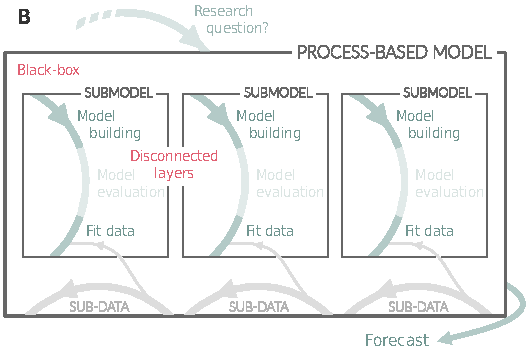
\includegraphics[width=\linewidth]{figures/forecasting_details}

    % \vspace{-0.5cm}\captionsetup{font=footnotesize}\captionof{figure}{Caption}\label{fig:trends}
    \vspace*{1mm}
\end{minipage}

\noindent % Process-based models are built on explicit mathematical equations to describe (supposedly causal) relationships between environmental drivers and ecological responses. 
% They also often incorporate empirical relationships, particularly when knowledge is incomplete or when some processes are intentionally omitted. Processes are often represented at different nested spatiotemporal scales, depending on the underlying assumptions. 
Model development is the central step of the process-based workflow, typically requiring several years, yet it often remains opaque from an external perspective. The step of designing the model---translating knowledge and hypotheses into mathematical equations and parameters---is often blurred with the step of model calibration (or tuning), where parameter values are inferred. Models are often treated as an accumulation of multiple submodels, each governing one or several ecological processes. Rather than being fitted as a whole, submodels are calibrated separately against specific subsets of data, and some parameters are simply prescribed (i.e. fix to a value found in the literature) or tuned to reproduce some observations or theory. The way models are currently calibrated is not a coincidence, but rather an inappropriate way to accommodate their complexity, where many parameters compensate for one another. % jdavies15april: is this more specific to process based  models? [FLAG: hmm yes again? Same point as above, maybe it's not clear we're talking mostly about PBM?]

\vfill

\end{multicols}}

\centerline{\bf A common workflow to bridge trend estimation and forecasting} % jdavies15april: would it be possible to label this panel with components of the LPI to provide a clearer illustration of how the framework is implemented? % [FLAG: not sure I understood]
\vspace*{-3mm}
{\begin{multicols}{2}
\begin{minipage}[t]{\linewidth}
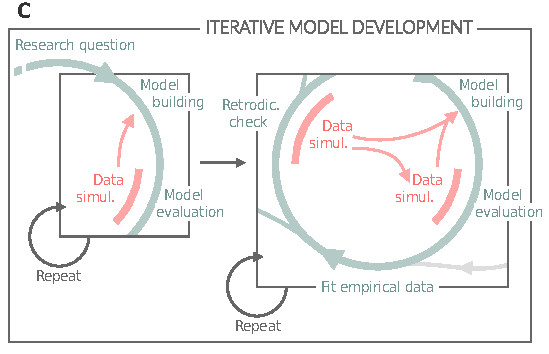
\includegraphics[width=\linewidth]{figures/iterativeworkflow_details}
    
% \vspace{-0.5cm}\captionsetup{font=footnotesize}\captionof{figure}{Caption}\label{fig:trends}
\vspace*{1mm}
\end{minipage}

\columnbreak
\vspace*{1mm}
Blabla... \\
% We say here briefly how great the new approach is or something.
An universal workflow offers an opportunity to bridge statistical and process-based frameworks, integrating mechanistic knowledge and leveraging robust statistical approaches \citep[e.g.][]{rounce2020quantifying}. Process-based models would no longer be perceived as deterministic black boxes by other researchers but rather as robust statistical frameworks encapsulating both data structure and mechanistic knowledge. And it would also be an opportunity to spread the incorporation of mechanistic assumptions beyond the process-based modeling community.

\end{multicols}}

\end{tcolorbox}

\section{Barriers and opportunities}

We believe our workflow could help advance ecological science and its applications, but widespread use of it requires overcoming major hurdles that pervade science.  
% One well-known hurdle is the pressure to publish, which can lower research standards and make the added effort of this workflow seem ill-placed. This may be especially true for those who see science rewarded mostly through the shear number of publications. But for those more focused on the long-term value of their work---for example, how well cited their papers are over a longer-time scale---we think this workflow can help. % jdavies15april: I am not sure this needs to be said, but could mention good model fitting takes time and is an iterative and learning process.
Good model fitting is inherently iterative and takes time, at odds with the pressure to publish quickly.
Further, growing concerns about how reproducible science is, especially in ecology where samples sizes are low and effects likely non-linear and complex, we believe adopting the workflow will pay off in the longer term, as more value is placed on research that carefully developed, openly shared (for data and code) and acknowledges its uncertainty towards the aim of improving future data collection and model development (see Fig). 

\subsection{Adopting the workflow}

Advancing ecology to where most researchers use models built more flexibly from ecological theory and insights applied to their ecological systems will not happen rapidly without a major shift in training. Much of ecology still divides the world into training for those focused on several groups: those who gather data and learn a limited set of pre-built models versus those who develop more complex models. In ecological training today researchers who conduct field and lab studies often learn a highly limited set of particular tests matched to particular experiment designs and simple information on their variable types (e.g., categorical $x$ and $y$ leads to using a chi square test). 

Instead, ecologists trained in a limited set of tests are expected to collaborate with others when they need more complex models, who were trained more in model development (though often for highly specific applications, such as wildlife population estimates, where they may rarely develop entirely new generative models). These two groups further differ from process-based modelers, who often train in physical and ecophysiological processes and how to abstract them into mainly deterministic models. % process-based modelers---often with a physical or ecophysiological background---mostly focus on simulating some mechanisms 
Few of these groups have integrated data simulation into their statistical or scientific workflows, which is generally reserved as a form of training needed mainly by those specializing in theoretical ecology, who often solve analytical equations but rarely link to empirical data. While specialization is valuable, we argue the fundamental % training 
separation in ecology has overly-siloed these groups and prevented more rapid progress.

Instead of training some ecologists extensively in experimental design and tests that may match certain designs (though rarely do for ecological data, CITES), training in the workflow would focus on learning to generate questions and then models, and then to simulate data from them. This would mean training all ecologists to link the ecological processes they study with the mathematical models that may describe them. Through this and retrodictive checks most ecologists would more easily think through what parameters are most critical to their question and or aim (e.g., management) and also gain a much stronger connection to the level of uncertainty in many of ecological estimates. Empirical ecologists would be more likely to recognize critical gaps in current models fit by those specializing in ecological modeling and help advance those models. Process-based modelers may start a new generation of simpler models that are more tractable to theoretical ecologists, who may suddenly see bridges from their work to empirical data and forecasting. 
% Perhaps the only drawback would be to those focused on statistical models, whose gate-keeping would suddenly fail them and they would have to do more that just say how amazing they are... 
Those focused on learning complex statistical models may find many of the field now share their excitement and interest in more generative models, and could focus on adapting approaches for better parameter estimation and improved forecasts.

\subsection{A tractable alternative to machine learning}

In a world where machine learning is rapidly advancing, there is no point of sticking to traditional methods if no changes are made. Machine learning will likely surpass process-based models if the latter lack a robust estimation of their parameters and fall in a complexity trap, at the cost of their interpretability. Similarly, trend analysis, when the focus is on methodological controversies (due to the lack of an iterative workflow) rather than on a robust mechanistic foundation, offers no clear advantage over machine learning. % jdavies15april: nothing intrinsically bad about ML, but sometimes the goal is just to understand the system, not make predictions or forecasts.

% jdavies15april: This could be the Concluding section highlighting the general advances provided by adopting your framework (and perhaps a better place for text currently at end of section 3.2).
Today model development in ecology is rarely transparent, which limits how easily the research community can understand modes, and thus identify potential issues. Instead of broad inclusive conversations about how to improve models to advance our ecological understanding, a significant portion of scientific debate today has become lost in methodological considerations, but we believe our workflow provides an tractable step to fixing this. By focusing on model development more tightly tied to ecological expertise, we ague this workflow should broader the community that contributes to model development. As ecologists are increasingly expanding their computational toolkits, many field, and lab and other forms of `empirical' ecologists have the basic tools to follow this workflow to build models that better represent their ecological, and---most importantly---to interrogate them.

\clearpage
\bibliography{forecastflows}

\end{document}